% Options for packages loaded elsewhere
\PassOptionsToPackage{unicode}{hyperref}
\PassOptionsToPackage{hyphens}{url}
\PassOptionsToPackage{dvipsnames,svgnames,x11names}{xcolor}
%
\documentclass[
  12pt]{article}

\usepackage{amsmath,amssymb}
\usepackage{lmodern}
\usepackage{iftex}
\ifPDFTeX
  \usepackage[T1]{fontenc}
  \usepackage[utf8]{inputenc}
  \usepackage{textcomp} % provide euro and other symbols
\else % if luatex or xetex
  \usepackage{unicode-math}
  \defaultfontfeatures{Scale=MatchLowercase}
  \defaultfontfeatures[\rmfamily]{Ligatures=TeX,Scale=1}
\fi
% Use upquote if available, for straight quotes in verbatim environments
\IfFileExists{upquote.sty}{\usepackage{upquote}}{}
\IfFileExists{microtype.sty}{% use microtype if available
  \usepackage[]{microtype}
  \UseMicrotypeSet[protrusion]{basicmath} % disable protrusion for tt fonts
}{}
\makeatletter
\@ifundefined{KOMAClassName}{% if non-KOMA class
  \IfFileExists{parskip.sty}{%
    \usepackage{parskip}
  }{% else
    \setlength{\parindent}{0pt}
    \setlength{\parskip}{6pt plus 2pt minus 1pt}}
}{% if KOMA class
  \KOMAoptions{parskip=half}}
\makeatother
\usepackage{xcolor}
\setlength{\emergencystretch}{3em} % prevent overfull lines
\setcounter{secnumdepth}{5}
% Make \paragraph and \subparagraph free-standing
\ifx\paragraph\undefined\else
  \let\oldparagraph\paragraph
  \renewcommand{\paragraph}[1]{\oldparagraph{#1}\mbox{}}
\fi
\ifx\subparagraph\undefined\else
  \let\oldsubparagraph\subparagraph
  \renewcommand{\subparagraph}[1]{\oldsubparagraph{#1}\mbox{}}
\fi

\usepackage{color}
\usepackage{fancyvrb}
\newcommand{\VerbBar}{|}
\newcommand{\VERB}{\Verb[commandchars=\\\{\}]}
\DefineVerbatimEnvironment{Highlighting}{Verbatim}{commandchars=\\\{\}}
% Add ',fontsize=\small' for more characters per line
\usepackage{framed}
\definecolor{shadecolor}{RGB}{241,243,245}
\newenvironment{Shaded}{\begin{snugshade}}{\end{snugshade}}
\newcommand{\AlertTok}[1]{\textcolor[rgb]{0.68,0.00,0.00}{#1}}
\newcommand{\AnnotationTok}[1]{\textcolor[rgb]{0.37,0.37,0.37}{#1}}
\newcommand{\AttributeTok}[1]{\textcolor[rgb]{0.40,0.45,0.13}{#1}}
\newcommand{\BaseNTok}[1]{\textcolor[rgb]{0.68,0.00,0.00}{#1}}
\newcommand{\BuiltInTok}[1]{\textcolor[rgb]{0.00,0.23,0.31}{#1}}
\newcommand{\CharTok}[1]{\textcolor[rgb]{0.13,0.47,0.30}{#1}}
\newcommand{\CommentTok}[1]{\textcolor[rgb]{0.37,0.37,0.37}{#1}}
\newcommand{\CommentVarTok}[1]{\textcolor[rgb]{0.37,0.37,0.37}{\textit{#1}}}
\newcommand{\ConstantTok}[1]{\textcolor[rgb]{0.56,0.35,0.01}{#1}}
\newcommand{\ControlFlowTok}[1]{\textcolor[rgb]{0.00,0.23,0.31}{#1}}
\newcommand{\DataTypeTok}[1]{\textcolor[rgb]{0.68,0.00,0.00}{#1}}
\newcommand{\DecValTok}[1]{\textcolor[rgb]{0.68,0.00,0.00}{#1}}
\newcommand{\DocumentationTok}[1]{\textcolor[rgb]{0.37,0.37,0.37}{\textit{#1}}}
\newcommand{\ErrorTok}[1]{\textcolor[rgb]{0.68,0.00,0.00}{#1}}
\newcommand{\ExtensionTok}[1]{\textcolor[rgb]{0.00,0.23,0.31}{#1}}
\newcommand{\FloatTok}[1]{\textcolor[rgb]{0.68,0.00,0.00}{#1}}
\newcommand{\FunctionTok}[1]{\textcolor[rgb]{0.28,0.35,0.67}{#1}}
\newcommand{\ImportTok}[1]{\textcolor[rgb]{0.00,0.46,0.62}{#1}}
\newcommand{\InformationTok}[1]{\textcolor[rgb]{0.37,0.37,0.37}{#1}}
\newcommand{\KeywordTok}[1]{\textcolor[rgb]{0.00,0.23,0.31}{#1}}
\newcommand{\NormalTok}[1]{\textcolor[rgb]{0.00,0.23,0.31}{#1}}
\newcommand{\OperatorTok}[1]{\textcolor[rgb]{0.37,0.37,0.37}{#1}}
\newcommand{\OtherTok}[1]{\textcolor[rgb]{0.00,0.23,0.31}{#1}}
\newcommand{\PreprocessorTok}[1]{\textcolor[rgb]{0.68,0.00,0.00}{#1}}
\newcommand{\RegionMarkerTok}[1]{\textcolor[rgb]{0.00,0.23,0.31}{#1}}
\newcommand{\SpecialCharTok}[1]{\textcolor[rgb]{0.37,0.37,0.37}{#1}}
\newcommand{\SpecialStringTok}[1]{\textcolor[rgb]{0.13,0.47,0.30}{#1}}
\newcommand{\StringTok}[1]{\textcolor[rgb]{0.13,0.47,0.30}{#1}}
\newcommand{\VariableTok}[1]{\textcolor[rgb]{0.07,0.07,0.07}{#1}}
\newcommand{\VerbatimStringTok}[1]{\textcolor[rgb]{0.13,0.47,0.30}{#1}}
\newcommand{\WarningTok}[1]{\textcolor[rgb]{0.37,0.37,0.37}{\textit{#1}}}

\providecommand{\tightlist}{%
  \setlength{\itemsep}{0pt}\setlength{\parskip}{0pt}}\usepackage{longtable,booktabs,array}
\usepackage{calc} % for calculating minipage widths
% Correct order of tables after \paragraph or \subparagraph
\usepackage{etoolbox}
\makeatletter
\patchcmd\longtable{\par}{\if@noskipsec\mbox{}\fi\par}{}{}
\makeatother
% Allow footnotes in longtable head/foot
\IfFileExists{footnotehyper.sty}{\usepackage{footnotehyper}}{\usepackage{footnote}}
\makesavenoteenv{longtable}
\usepackage{graphicx}
\makeatletter
\def\maxwidth{\ifdim\Gin@nat@width>\linewidth\linewidth\else\Gin@nat@width\fi}
\def\maxheight{\ifdim\Gin@nat@height>\textheight\textheight\else\Gin@nat@height\fi}
\makeatother
% Scale images if necessary, so that they will not overflow the page
% margins by default, and it is still possible to overwrite the defaults
% using explicit options in \includegraphics[width, height, ...]{}
\setkeys{Gin}{width=\maxwidth,height=\maxheight,keepaspectratio}
% Set default figure placement to htbp
\makeatletter
\def\fps@figure{htbp}
\makeatother

\addtolength{\oddsidemargin}{-.5in}%
\addtolength{\evensidemargin}{-1in}%
\addtolength{\textwidth}{1in}%
\addtolength{\textheight}{1.7in}%
\addtolength{\topmargin}{-1in}%
\makeatletter
\makeatother
\makeatletter
\makeatother
\makeatletter
\@ifpackageloaded{caption}{}{\usepackage{caption}}
\AtBeginDocument{%
\ifdefined\contentsname
  \renewcommand*\contentsname{Table of contents}
\else
  \newcommand\contentsname{Table of contents}
\fi
\ifdefined\listfigurename
  \renewcommand*\listfigurename{List of Figures}
\else
  \newcommand\listfigurename{List of Figures}
\fi
\ifdefined\listtablename
  \renewcommand*\listtablename{List of Tables}
\else
  \newcommand\listtablename{List of Tables}
\fi
\ifdefined\figurename
  \renewcommand*\figurename{Figure}
\else
  \newcommand\figurename{Figure}
\fi
\ifdefined\tablename
  \renewcommand*\tablename{Table}
\else
  \newcommand\tablename{Table}
\fi
}
\@ifpackageloaded{float}{}{\usepackage{float}}
\floatstyle{ruled}
\@ifundefined{c@chapter}{\newfloat{codelisting}{h}{lop}}{\newfloat{codelisting}{h}{lop}[chapter]}
\floatname{codelisting}{Listing}
\newcommand*\listoflistings{\listof{codelisting}{List of Listings}}
\makeatother
\makeatletter
\@ifpackageloaded{caption}{}{\usepackage{caption}}
\@ifpackageloaded{subcaption}{}{\usepackage{subcaption}}
\makeatother
\makeatletter
\@ifpackageloaded{tcolorbox}{}{\usepackage[many]{tcolorbox}}
\makeatother
\makeatletter
\@ifundefined{shadecolor}{\definecolor{shadecolor}{rgb}{.97, .97, .97}}
\makeatother
\makeatletter
\makeatother
\ifLuaTeX
  \usepackage{selnolig}  % disable illegal ligatures
\fi
\usepackage[]{natbib}
\bibliographystyle{agsm}
\IfFileExists{bookmark.sty}{\usepackage{bookmark}}{\usepackage{hyperref}}
\IfFileExists{xurl.sty}{\usepackage{xurl}}{} % add URL line breaks if available
\urlstyle{same} % disable monospaced font for URLs
\hypersetup{
  pdftitle={Introductory Data Science: A Blueprint to Navigate Curricular, Pedagogical, and Computational Challenges},
  pdfauthor={Elijah Meyer; Mine Çetinkaya-Rundel},
  pdfkeywords={Data Science, Curriculum, Pedagogy},
  colorlinks=true,
  linkcolor={blue},
  filecolor={Maroon},
  citecolor={Blue},
  urlcolor={Blue},
  pdfcreator={LaTeX via pandoc}}


\begin{document}


\def\spacingset#1{\renewcommand{\baselinestretch}%
{#1}\small\normalsize} \spacingset{1}


%%%%%%%%%%%%%%%%%%%%%%%%%%%%%%%%%%%%%%%%%%%%%%%%%%%%%%%%%%%%%%%%%%%%%%%%%%%%%%

\date{May 3, 2023}
\title{\bf Introductory Data Science: A Blueprint to Navigate
Curricular, Pedagogical, and Computational Challenges}
\author{
Elijah Meyer\\
Department of Statistics, Duke University\\
and\\Mine Çetinkaya-Rundel\\
Department of Statistics, Duke University\\
}
\maketitle

\bigskip
\bigskip
\begin{abstract}
The text of your abstract. 200 or fewer words.
\end{abstract}

\noindent%
{\it Keywords:} Data Science, Curriculum, Pedagogy
\vfill

\newpage
\spacingset{1.9} % DON'T change the spacing!
\ifdefined\Shaded\renewenvironment{Shaded}{\begin{tcolorbox}[sharp corners, breakable, enhanced, borderline west={3pt}{0pt}{shadecolor}, boxrule=0pt, frame hidden, interior hidden]}{\end{tcolorbox}}\fi

\hypertarget{introduction}{%
\section{Introduction}\label{introduction}}

The demand for trained data scientists is putting pressure on
instructors to create and advance the teachings of such courses. An
estimated 11.5 million new data science jobs are projected to be created
by 2026, while employment of data scientists is projected to grow by 36
percent from 2021 to 2031 \citep{labor_2022}. As demand increases, class
sizes to best prepare students for these positions increase as well. The
increasing volume of enrollment of data science students
\citep{Redmond2022} requires that statistics and data science educators
commit to developing modern curriculum in order to help students be
successful. Despite the demand, academics are still struggling with what
a modern data science curriculum should look like \citep{Schwab2020},
and how it can be effectively taught to a large student audience. To
this point, much more thought, work, and discussions need to take place
before a consensus is reached on what a modern data science curricula
should look like.

To answer this call, the Curriculum Guidelines for Undergraduate
Programs in Data Science provided six major recommendations as to what
practitioners of data science should be competent in: computational and
statistical thinking, mathematical foundations, model building and
assessment, algorithms and software foundation, data curation, knowledge
transference---communication and responsibility \citep{veaux_2017}.
Additionally, the Association for Computing Machinery Education
Council's Data Science Task Force explores and expands
discipline-specific conversations around the field of data science
{[}\citet{Danyluk_2021}. This task force acknowledges that data science
curricula can be flexible, but suggests that data science curricula
should include applications designed towards building skills in
computing, statistics, machine learning and mathematics.

However, there currently lacks alignment between such recommendations
and what is observed in practice, with the majority of context across
the landscape of data science curricula largely focusing on how to model
data \citep{Donoho2017} \textbf{TO DO: Rephrase sentence, I wasn't sure
what's meant here}. The picture becomes even less clear on what context
constitutes a well developed modernized introductory data science
course. This presents a need for a \emph{blueprint} to design and
implement and modernized introduction to data science course that lays
the foundation for students to develop an encompassing data science
skill set. In this paper, we lay out this blueprint, while addressing
realistic challenges, instructors may face when developing, creating,
and implementing an introductory data science course. This discussion is
through the lens of a modernized data science curricula for an
introductory data science course at Duke University \textbf{TO DO:
Implement blinding}.

This course is designed for large class sizes that enrolls students with
little to no statistics, data science, or coding experience, common
hurdles identified by faculty when trying to implement a data science
course \citep{Schwab2020}. By the end of this course, students are
expected and able to clean, investigate, and communicate with data in a
reproducible manner while answering a targeted research question.
Detailed learning objectives of this course include learning to explore,
visualize, and analyze data in a reproducible and shareable manner
through the use of R-studio and GitHub \citep{R21, github}. Through
these programs, students gain experience in data wrangling, exploratory
data analysis, predictive modeling, and data visualization. These
experiences are generated through the \emph{Kaplan Way}. The Kaplan Way
is a learning model ``that combines a scientific, evidence-based design
philosophy with a straightforward educational approach to learning''
\citep{schweser_2023}. This learning model posits a three-phase learning
strategy: Prepare, Practice, and Perform \textbf{TO DO: Check in with
Maria about provenance of PPP}. During each of these phases, students
are equipped with the appropriate tools to acquire knowledge, be given
an opportunity to apply what they know, and to demonstrate mastery of
the tasks at hand.

In this paper, we discuss the creation and implementation of curricular
and pedagogical decisions made in designing the introductory data
science course at Duke University. This includes detailing the
implementation of the Kaplan Way learning model, to support a large
class of students with a diverse background in statistics, data science,
and coding experience. Within this format, we provide examples of and
describe activities and assessments given both in and outside of class.
We extend discussions and provide recommendations for implementing and
integrating computing tools, such as R-studio and GitHub, through our
experiences in our course. Lastly, we discuss challenges, and provide
insight to help instructors wanting to adopt or adapt a course similar
to introductory to data science at Duke University. The purpose of this
paper is to continue the discussion, and present a modernized curricula
for an introductory data science course at Duke University, and the
pedagogical decisions to help best equip students with the data science
skills necessary for future classes.

\hypertarget{sec-course}{%
\section{The Course}\label{sec-course}}

In the following sections, we describe our introductory data science
course, offered to predominantly freshman level students at Duke
University, titled Introduction to Data Science and Statistical Thinking
(STA199). Often, these students are \textbf{(interested in / major +
minor in / description of typical student demographic) TO DO: Look in
the getting to know you survey?}. Students enrolling in STA199 commonly
have little to no statistics, data science, or coding experience. In a
typical semester, this course seats roughly 179 students, which is
considered to be large by all measures. Both the lack of experience and
large class size are identified as two common hurdles by faculty when
trying to create and instruct an introductory data science course
\citep{Schwab2020, Kok_2008}. However, by the end of this course,
students are able to use data both the statistical software R and GitHub
to create data visualizations, investigate patterns, and model outcomes
in a reproducible format.

This course is built on four large-scale learning objectives: learn to
explore, visualize and analyze data in a reproducible and shareable
manner; gain experience in data wrangling and munging, exploratory data
analysis, predictive modeling, and data visualization; work on problems
and case studies inspired by and based on real-world questions and data;
learn to effectively communicate results through written assignments and
project presentation. These objectives are accomplished through
interactive lectures and labs that present content, problems, and case
studies inspired by and based on real-world questions and data.

When teaching, instructors are committed to the Kaplan Way learning
model (Figure 1) ``that combines a scientific, evidence-based design
philosophy with a straightforward educational approach to learning''
\citep[pg. 3]{schweser_2023}.

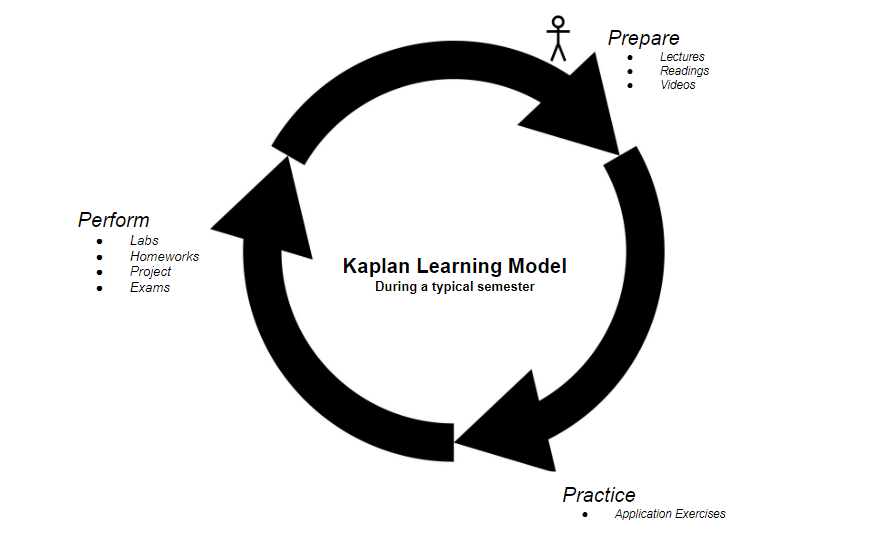
\includegraphics{images/Kaplan.png} \textbf{Fig 1:} Kaplan Learning
Model for STA 199

This model is composed of three phases: prepare, practice, and perform.
All three phases are designed to guide the instructor in facilitating an
overall quality learning experience for the student. Each of these
phases are performed during a typical week within a semester,
accomplished through preparation materials, lectures, in-class
application exercises (AEs), labs, and assessments.

During the prepare phase, students are completing readings, watching
videos, and listening to lectures. These modes of learning ultimately
helps students' develop a new foundation of data science concepts. The
goal of the prepare phase is to put students in a position where they
can build upon what they are learning, and create new knowledge through
the practice phase. The practice phase is designed to be an opportunity
for students to reinforce the new information gained, as well as uncover
new concepts in data science. This is achieved through the use of
interactive AEs administered in class where students either work alone,
in groups, or with the instructor in live coding sessions. Finally,
students enter the perform phase, showcasing their progress made in the
previous two phases. This is typically done through assessments such as
homework, labs, exams, and projects. This learning model is a continuous
cycle throughout the semester as new topics are introduced.

Topics taught through this cycle fall under two major units: Unit 1 -
Exploring data; Unit 2 - Making rigorous conclusions. In Unit 1,
students become first introduced to R, R-studio, and Github. During this
unit, students start to create data visualizations and learn how to both
import and manipulate data to be better suited for modeling. In Unit 2,
students extend their investigations with data to include modeling.
Specifically, students fit a variety of models (simple linear
regression, multiple linear regression, logistic regression), and learn
the fundamentals of hypothesis testing and confidence intervals. For a
more complete description of the topics taught and data sets used in
creating these lessons, please see \emph{A fresh look at introductory
data science} \citep{Cetinkaya2020}. \textbf{TO DO: See updated unit
breakdown in data science in a box.}

In this paper, we describe the preparation and implementation process
necessary to run STA199, in its entirety. This includes details of a
teaching team used to instruct, technology we've chosen to use, as well
as our pedagogical choices that go into a typical week of teaching. This
comprehensive description is encouraged to be used as a flexible
framework on how to create, set up, and implement an introduction to
data science course similar to STA199. In this description, we
articulate first hand experiences, suggestions, and provide example code
and lessons that aim to support newer instructors who are developing or
teaching an introductory data science course; instructors with courses
that are increasing in size; and instructors who want to implement more
technical tools into their curricula and classroom.

\hypertarget{teaching-team}{%
\section{Teaching Team}\label{teaching-team}}

We structure a teaching team to help account for the difficulties a
large class size can bring. Our teaching team consists of one instructor
and multiple teaching assistants (TAs). The responsibilities of any TA
is to both support the instructor in charge of the class, and support
the students in the classroom. These TAs range from undergraduate to
PH.D. level students, and vary in teaching experience. \textbf{(Writing
on TA selection process). Once selected\ldots{} (writing on TA
training).}

Once training is complete, TAs are assigned roles that indicate their
responsibilities during the semester. These roles include \emph{course
organizer}, \emph{head TA}, \emph{lab leader}, and \emph{lab helper}.
Often, these roles are given based on the academic level of student,
with more academically experienced TAs taking on the roles of course
organizer, head TA, and lab leader, where as students with less
experience (i.e.~undergraduate students) take on the role of lab helper.

Lab sections are held once a week, and are facilitated in person by both
a lab leader and lab helper. The responsibilities of a lab helper are
supporting both the students and lab leader as they see fit. Examples of
this may include setting up the classroom before class, or conducting
small group conversations when students have questions about the
material. The lab leader is responsible for facilitating the lab. This
may involve giving a brief introduction and wrap up of lab content, as
well as being able to answer questions and facilitate conversations
among students about the lab assessment material. In addition, both must
hold two hours of office hours each week and have grading
responsibilities assigned throughout the semester.

Head TA responsibilities can generally be categorized into the following
categories: Administrative and pedagogical. Administrative
responsibilities include the organization and distribution of TA
responsibilities throughout the semester. It is imperative that the head
TA and instructor clearly communicate expectations with each other to
establish exactly how rules and responsibilities are assigned to TAs.
This includes distributing grading assignments and deadlines to both lab
helpers and leaders, weekly. The head TA also makes sure that all TAs
complete grading within a week and spot check the grading accuracy and
quality of all written feedback given. Other administrative duties
include reminding other TAs about bi-weekly payroll deadlines and ensure
TAs are working their alloted hours per week (and not more).
Pedagogically, head TAs are responsible for creating or reviewing answer
keys and grading rubrics for homework and lab assessments as the
instructor sees fit. Each head TA is also assigned to instruct one lab
section during the semester. Before becoming a Head TA, there is
additional training that specializes head TAs in their administrative
responsibilities.

The course organizer is expected to work across each section of STA199,
instead of working with a single instructor. Their responsibilities
include creating rubrics for and working through homework and lab
assignments. Additionally the course organizer, along with the
instructor, answers real time questions virtually during labs asked by
lab leaders. Questions often range from content related to technical
questions about GitHub and R. Finally, the course organizer is
responsible for handling all requested assignment extensions from
students. This includes filing away student exemptions, providing
extensions for extreme circumstances, and enforcing the late work policy
outlined in the syllabus when necessary.

We typically have one course organizer, one head TA, six lab leaders,
and six lab helpers. Although this is our proposed team structure, we
want to emphasize that there is great flexibility in coming up with how
a teaching team is built and operates for an introductory to data
science course. Among any team, we encourage a system designed to
alleviate the grading responsibilities of a large class from a single
individual, dispersed into many among the team. When grading, it is
suggested that each individual is properly trained on how to grade
assessments, and expectations on how to provide feedback are clear.
Unclear feedback given has often been a point of contention from
students in the past. For each assignment, we recommend having one
member of the team grade one problem across the entirety of the class
roster. This helps adhere to more consistent grading, and encourages
more grading questions to be asked as they arise, earlier in the grading
process.

Through our experiences, it has been imperative that everyone within the
team is communicating with each other. A team with many different roles
poses risk for the instructor to be unaware of how or what decisions are
being enacted at the grading and lab levels of the course. Thus, it is
recommended that the instructor trains everyone on the teaching team to
use a communication system that allows every member to communicate any
questions they may have, or decisions they make, to the entire team. In
the past, we have used the software \emph{Slack}, with appropriately
named channels such as \emph{grading-questions}, where TAs can post
grading examples and questions about grading so the instructor can
clearly respond with their expectations. Further, it should be noted
that the head TA should not be treated as a ``bridge of communication''
for the instructor to the rest of the teaching team. It is critical that
that the instructor is in consistent contact with all members of the
teaching team in making sure all lab leaders and helpers understand the
course content, how to grade, and know what's expected of them in their
assigned role. We recommend holding a weekly meeting with all members of
the teaching team to ensure this. When members are unable to come, it is
an expectation that they watch a recorded video of the meeting and reach
out if they have any questions about what was discussed.

\hypertarget{sec-tech}{%
\section{Technology}\label{sec-tech}}

We use R, R-studio, and GitHub to create interactive lessons, and assign
pre-created assessments to individual or groups of students. In the
following sections, we detail the computing infrastructure needed to do
so. This includes details and examples with R, R-studio, and GitHub,
from the instructor's perspective, to set up lectures, AEs, labs and
homework. First, we justify our decision to use GitHub in STA199 before
detailing necessary steps and student information needed so creation can
take place.

\hypertarget{why-github}{%
\subsection{Why GitHub}\label{why-github}}

We choose to use GitHub for STA199 because it easily and efficiently
allows us to create and administer assessments and interactive lessons
to a large class size in individual GitHub repositories. Further, within
these repositories, instructors can provide template code and other
resources necessary to best facilitate an interactive lesson where
students can code together with the instructor during lecture.
Additionally, teaching through GitHub provides the ability to re-use
what you currently create as a template for subsequent semesters. Thus,
this system both rewards and encourages time investment into the
creation of assessments and lesson plans. Moreover, exposing students to
version control software early in their academic career helps them
develop good habits as researchers and emphasize the importance of
reproducibility in science. These are just some of the many benefits of
using GitHub in an introductory data science course. To take advantage
of these benefits as an instructor, we first need students to create
their own GitHub account.

\hypertarget{setting-up-a-github-account}{%
\subsection{Setting up a GitHub
account}\label{setting-up-a-github-account}}

To participate in interactive lessons and assessments, students must set
up a GitHub account. This is done of the first day of class, and often,
students are given time during class to sign up. Following tips from
``Happy Git with R'' \citep{bryan_hester_2020}, we suggest students do
the following when creating their name:

-- Incorporate their actual name

-- Reuse their username from other contexts if you can

-- Pick a username they will be comfortable revealing to a future boss

-- Be as unique as possible in as few characters as possible. Shorter is
better than longer

-- Avoid words with special meaning in programming (i.e., NA)

Once students create their account, we suggest getting this information
from them in a survey. This normally can be done through your learning
management system. It is critical to reiterate to students that spelling
and capitalization matter when they provide their GitHub username. We
suggest asking the question as follows:

\textbf{(should we include the questions in a highlighted text box of
some sort?)}

\textbf{What is your GitHub username?}

\textbf{Answer this question by ONLY typing your GitHub name and nothing
else.}

\textbf{Make sure you triple-check the spelling so I don't add random
strangers to our course organization on GitHub}

Once this information is collected, it must be exported and stored as a
\texttt{.csv} file to be read into R later. We recommend having the
following structure of data collected from the survey.

\begin{longtable}[]{@{}lll@{}}
\toprule()
\endhead
last\_name & first\_name & github\_username \\
& & \\
\bottomrule()
\end{longtable}

\textbf{Fig 2: Example Data Collection}

If you, as the instructor, do not have a GitHub account, you will need
to create one as well. This student information will be used to enroll
students in your created GitHub organization for your course.

\hypertarget{github-organization}{%
\subsection{GitHub organization}\label{github-organization}}

GitHub organizations are shared accounts where instructors and students
can collaborate across many projects at once. Using your GitHub account,
you can create a new GitHub organization by clicking on your profile
icon in the upper right hand corner, clicking \emph{Settings},
\emph{Access}, \emph{New Organization}. It's suggested to name this
organization the name of your class and the current semester you
teaching in (i.e., sta199-s23). Once your organization is created, you
can use packages within R and R-studio to invite students to enroll.
Once enrolled, we can create and efficiently distribute assessments and
live coding activities for them to access on their own laptop device.

\hypertarget{why-r-r-studio}{%
\section{Why R \& R-Studio}\label{why-r-r-studio}}

R is a statistical programming language for computing and modeling while
R-studio is an integrated development environment for R \citep{Rcite}.
We choose these resources because they are freely available to download
and are in high demand in different data science job opportunities
\textbf{(cite?)}. In addition, this programming language has a
comprehensive library of packages that allows students to create data
visualizations and seamlessly analyze data, aligning with our learning
objectives for the course. Further, this software is compatible with
online versions that students can access without having to go through a
local installment if they do not wish or are unable. There exists online
versions that can be set up for students, with capabilities of
pre-populating their software with the appropriate packages needed for
the semester. Addressing these hurdles for students early is
advantageous any instructor who is working with a large amount of
students that are inexperienced with coding.

\hypertarget{setting-up-students-r-r-studio}{%
\subsection{Setting Up Students R \&
R-Studio}\label{setting-up-students-r-r-studio}}

In an introductory course, it is recommended to minimize student
frustration and distraction through the use of pre-packaged
computational infrastructure \citep{Rundel2018}. Per this
recommendation, STA199 has students use R and R-studio through a
\emph{Duke Container}. Duke containers provides instructors at Duke
university the opportunity to facilitate the use of different software,
such as R and R-studio, through an online container instead of needing
students to locally download both programs. Additionally, instructors
have the ability to manage and install packages students will need for
the semester, helping provide a neat and well organized starting
experience with a new statistical language. \textbf{(insert discussion
on how this is done)}.

\textbf{(Transition to R-studio cloud discussion? What alternatives can
instructors use to imitate Duke containers if this is something they do
not have access to at their university.)}

\hypertarget{using-r-r-studio-to-manage-github-organization}{%
\subsection{Using R \& R-Studio to Manage GitHub
organization}\label{using-r-r-studio-to-manage-github-organization}}

To invite students into your GitHub organization, we will use a myriad
of functions from the \texttt{gh\_class} package. \textbf{(insert
discuss on what the gh-class package is).}

To start, we suggest creating a separate GitHub repository that will
contain all code used to invite students to your organization and to
create individual student repositories. Within a document in this new
repository, we must first define our GitHub organization as a character
string to be used in later function. We suggest calling this
\texttt{org}.

\begin{Shaded}
\begin{Highlighting}[]
\NormalTok{org }\OtherTok{\textless{}{-}} \StringTok{"sta{-}199{-}s23"}
\end{Highlighting}
\end{Shaded}

The following code below invites students to your GitHub organization
using your defined org and the GitHub usernames collected from your
students in a previous survey (see section Setting up a GitHub account).
For the example below, we chose to name the student survey data as
``roster.csv''.

\begin{Shaded}
\begin{Highlighting}[]
\CommentTok{\# invite students {-}{-}{-}{-}{-}{-}{-}{-}{-}{-}{-}{-}{-}{-}{-}{-}{-}{-}{-}{-}{-}{-}{-}{-}{-}{-}{-}{-}{-}{-}{-}{-}{-}{-}{-}{-}{-}{-}{-}{-}{-}{-}{-}{-}{-}{-}{-}{-}{-}{-}{-}{-}{-}{-}{-}{-}{-}{-}{-}{-}{-}{-}}

\NormalTok{roster }\OtherTok{\textless{}{-}} \FunctionTok{read\_csv}\NormalTok{(}\StringTok{"roster.csv"}\NormalTok{)}

\FunctionTok{org\_invite}\NormalTok{(}
  \AttributeTok{org =}\NormalTok{ org,}
  \AttributeTok{user =}\NormalTok{ roster}\SpecialCharTok{$}\NormalTok{gihub\_name}
\NormalTok{)}
\end{Highlighting}
\end{Shaded}

Once the invites are sent, students will need to accept the invitation
to the organization.

Streamlining your course through R, R-studio, and GitHub greatly
alleviates common challenges that arise when working with a large class
size, such as activity and assessment distribution. This includes the
creation and distribution of in-class AEs, lectures, labs, and homework
assignments.

In the following sections, we discuss pedagogy used within our course,
strategies on how to implement such pedagogy in the classroom, and
detail the creation and distribution of AEs and lab assessments using R,
R-studio, and GitHub during a typical week in the semester (Figure 2).

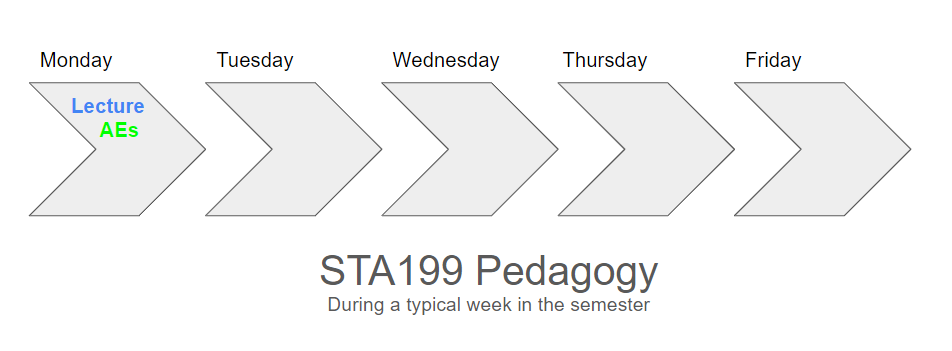
\includegraphics{images/pedagogy.png} \textbf{Fig 2:} Model of
pedagogical choices used in STA199 for a typical week

\hypertarget{sec-ped}{%
\section{Pedagogy}\label{sec-ped}}

In STA199, we have chosen a combination of teaching methods, interactive
activities, and learning assessments to help prepare introductory data
science students the tools they need to be successful outside of
university or in future coursework. Our pedagogy includes a combination
of lectures, facilitating in-class AEs, and running a lab, to provide
students an opportunity to perform what they've learned.

\hypertarget{lecture-application-exercises}{%
\subsection{Lecture \& Application
Exercises}\label{lecture-application-exercises}}

During a typical week in the semester, class is held twice a week. Class
is a combination of lecture and interactive AEs. The amount of time
dedicated to lecture and AEs can and should vary by instructor.
Typically, we allot the first 15 minutes of class for lecture. During
this time, students are introduced to new content that will be
re-addressed in the AE. To help maximize engagement of such a large
class size, we allot more class time to individual and team-based AEs
where students are asked to code on their own, together, or along with
the instructor. This is followed by a roughly 5-10 minute allotment for
a wrap up lecture, summarizing the highlights of AE.

Application exercises are structured interactive lessons that allow
students to learn through doing in class. Students are expected to bring
their laptops to class to participate in AEs. This expectation is made
clear prior to the first day of teaching. The purpose of these exercises
are to give students the opportunity to practice apply the statistical
concepts and code introduced in the prepare videos, readings, and
anything introduced during lecture.

When first starting to create an AE, we suggest streamlining the process
through a GitHub template repository cloned into R-studio as a project.
We choose to use \emph{Quarto}, within R-studio, to create AEs. This
choice is intentional, to provide students the opportunity to practice
writing code and answering questions in a reproducible format supported
by R and R-studio. When designing questions for an AE, we suggest
creating a mix of coding and concept questions (e.g., fill in the code
blanks, short response questions) that encourage students to follow
along with instructor demonstrations, and also provides students an
opportunity to answer questions on their own. This format has largely
been accepted and appreciated by students: ``I really enjoy the AE's and
that you take the time to walk us through the code and answer questions;
I like how the ae gives us a chance to practice the skills on our own
after class as well.'' Additionally, we suggest that questions are
scaffold, meaning that if students fall behind or type incorrect code
when trying to initially follow along, that they have access to correct
code that grants them the ability to continue engaging for the remaining
AE. This is especially important at the beginning of the semester to
minimize students' frustration around a new coding language. This may
include having answers to questions in a separate Quarto document that
students have access to, or within the same document as the AE.
Moreover, we suggest clearly labeling where students are expected to
type out answers in text or code throughout the exercise to further
streamline their involvement and continue to minimize frustration.

An example on an AE used to help teach \textbf{(insert concept)} can be
found here: \textbf{(insert example AE)}

We highly recommended designing lessons with built in time to have
students work on their own. The amount of time can largely depend on the
question being asked, and the teaching style of the instructor. We have
found that multiple 3-5 minute blocks for students to answer questions
without the instructor's guidance works well. This has been especially
effective if the code is then created together as a class, built off
student responses, to provide immediate feedback to students before
moving on to the next set of material or questions.

Once created, we can distribute this AEs to students within the class
GitHub organization by using the function
\texttt{org\_create\_assignment} from the \texttt{gh\_class} package.
Example code can be seen below.

\begin{Shaded}
\begin{Highlighting}[]
\NormalTok{assignment }\OtherTok{\textless{}{-}} \StringTok{"AE{-}5"} \CommentTok{\#name of AE repository you want to distribute }

\NormalTok{student\_name }\OtherTok{\textless{}{-}} \FunctionTok{org\_members}\NormalTok{(}\AttributeTok{org =}\NormalTok{ org, }\AttributeTok{include\_admins =} \ConstantTok{FALSE}\NormalTok{) }\CommentTok{\#name of students to create AE repository for}

\FunctionTok{org\_create\_assignment}\NormalTok{(}
  \AttributeTok{org =}\NormalTok{ org,}
  \AttributeTok{repo =} \FunctionTok{paste0}\NormalTok{(assignment, }\StringTok{"{-}"}\NormalTok{, student\_name),}
  \AttributeTok{user =}\NormalTok{ student\_name,}
  \AttributeTok{source\_repo =} \FunctionTok{paste0}\NormalTok{(org, }\StringTok{"/"}\NormalTok{, assignment)}
\NormalTok{)}
\end{Highlighting}
\end{Shaded}

It should be noted that, with such a large class size, \textbf{(time out
error discussion?).}

\textbf{(Code to create ``second batch of AEs'' if needed?)}

Hands on interactive AEs are the backbone of learning in STA199. We have
found that providing students with the opportunity to code in real-time
during class keeps them more engaged and eager to continue learning
about the material, versus simply lecturing for a 75-minute period. This
strategy has received positive feedback from students with varying
degrees of coding and statistics experience.

As highlighted in previous sections this system, streamlined through
GitHub, encourages time investment into the creation of AEs. Investing
time into AE creation provides a strong environment for current students
to learn, and sets a foundation for AEs to be re-tooled instead of
recreated in subsequent semesters. Future renditions of this course can
be modified from previous GitHub organizations efficiently, saving
instructors valuable time and energy before and during the semester.

AEs are designed to be a low stakes assessment where students can earn
full credit by completing in class. Typically, we make AEs worth
completion points that total to be 5\% of a student's end of semester
grade. For students that do not show up to class, we make AEs due three
days from when the AE was assigned. At the end of the semester, if
student's have completed 80\% of AEs, they earn a 100\% for their grade.
Students turn in AEs by pushing their answers within the AE document up
to their GitHub repository. There have been mixed responses from both
students and instructors on assigning a grade to AEs. Disadvantages
include not currently having an efficient way to implement a hard
deadline that students must adhere to, without removing push access from
their AE GitHub repository all-together. Further, if an instructor does
not finish an AE in class, students who did not attend class can be
easily confused on what's expected of them to complete. We suggest
tailoring the decision of grading of AEs to your individual course as
you see fit.

\hypertarget{labs}{%
\subsection{Labs}\label{labs}}

Labs for STA199 meet once a week for 75 minutes, and are facilitated by
lab leaders and lab helpers. The purpose of labs are to allow students
to apply concepts found in prepare material, lecture, and AEs, to
various data analysis scenarios. Lab section sizes are kept to around 30
students so each have more of an opportunity to converse with each
other, the lab leader, and lab helper, when working through the lab
assessment.

Much like AEs, the instructor or head TA creates and clones a lab GitHub
repository to all students that contains any information and any other
intangibles (like a data set) by changing the \texttt{assignment} object
in the above R code (see section Lecture \& Application Exercises) to be
the name of original lab GitHub repository. In the lab GitHub
repository, we choose to create a starter document with places for
students to write code under specific question numbers. The actual lab
assessment that this document corresponds to can be found on the class
website that is referenced during lab time.

Roughly one-third of the way into the semester, students are assigned to
groups to complete a class project. We suggest strategically assigning
groups based on a collection of the following information

\begin{itemize}
\item
  Declared or Intended Major
\item
  Year in School
\item
  Suggested times they work on school assignments
\end{itemize}

From our experience, groups who have significantly different years in
school across students have more friction, and tend to work less well
together than students that have more similar years in school.
Additionally, we highly suggest pairing up students that share common
interests using their intended or declared major in school. The class
project assigned is an open ended research project where the group
collectively decides on a project topic. We have found that students can
feel disengaged or left out of the group if they have different
interests than the others, and their interests are not reflected when
picking a project topic. When groups our assigned, each group during a
lab are tasked to come up with a team name. This team name will be the
name used to create their team repositories for the remaining labs. We
add this information as follows to the roster document.

\begin{longtable}[]{@{}llll@{}}
\toprule()
team\_name & last\_name & first\_name & github\_username \\
\midrule()
\endhead
& & & \\
\bottomrule()
\end{longtable}

From this point forward in the semester, we choose to have all labs be
completed as group work. Introducing group work during labs and through
a class project can help students learn from different perspectives,
practice their communication skills, and improve their problem solving
skills in the context of statistics and data science.

We can use these new data and change the code found in Lecture \&
Application Exercises section to create repositories for each team.

\begin{Shaded}
\begin{Highlighting}[]
\NormalTok{teams }\OtherTok{\textless{}{-}} \FunctionTok{read\_csv}\NormalTok{(}\StringTok{"roster.csv"}\NormalTok{)}

\FunctionTok{org\_create\_assignment}\NormalTok{(}
  \AttributeTok{org =}\NormalTok{ org, }\CommentTok{\# name of your organization}
  \AttributeTok{repo =} \FunctionTok{paste0}\NormalTok{(assignment, }\StringTok{"{-}"}\NormalTok{, teams}\SpecialCharTok{$}\NormalTok{team), }\CommentTok{\#name of the repo you are cloning and teams you are cloning for}
  \AttributeTok{user =}\NormalTok{ teams}\SpecialCharTok{$}\NormalTok{github\_username, }\CommentTok{\#adding individual students to team repo}
  \AttributeTok{team =}\NormalTok{ teams}\SpecialCharTok{$}\NormalTok{team\_name, }\CommentTok{\#team (or group) they are added to}
  \AttributeTok{source\_repo =} \FunctionTok{paste0}\NormalTok{(org, }\StringTok{"/"}\NormalTok{, assignment) }\CommentTok{\#naming repo }
\NormalTok{)}
\end{Highlighting}
\end{Shaded}

The new expectation is that once groups are formed, one lab assessment
will be turned in for each group instead of each individual. This
further helps lessen the grading responsibilities to those that are
assigned it.

After groups are formed, we give a set of recommendations for groups to
help promote a successful and positive group dynamic. This includes:

\begin{itemize}
\item
  Establish a clear line of communication with all members
\item
  Share ideas. Let your voice be heard.
\item
  Teach each other.
\item
  Do not approach group work as a bunch of individual assignments.
\end{itemize}

To further ensure positive group dynamic, we initiate three peer review
surveys. These peer review surveys provide insight into each group's
dynamic and may inform the teaching team of issues that may need to be
addressed. Questions within each survey range from having only having
instructor only visibility, to being shared with all team members to
promote productive conversations. An example question includes:
\emph{Estimate the percentage of the total amount of work/effort done by
each member, including yourself. Be sure your percentages sum to 100\%!}
We suggest adding additional questions as deemed necessary to help best
understand how everyone is working together within a group.

A new instructor of data science, or one with an increasing class size
should think critically if and how they want to implement group work in
their classroom. In our experience, merge conflicts, the number of
groups, and group formation have been the most difficult aspects of
facilitating group work. Students, especially those newer to coding, are
extremely hesitant to create merge conflicts. Despite a lab dedicated to
the creation and fixing of merge conflicts, students often express
frustration and feel as though they are doing something wrong when merge
conflicts occur. Some groups choose to collaborate using other forms of
technology (e.g., Google documents) before committing and pushing their
finished work onto GitHub. We highly advise against this, and try to
incentivise students by emphasizing the practical importance of learning
how to work through merge conflicts. Secondly, the sheer number of
groups created from 179 students creates an additional time investment
for all members of the teaching team. This includes making sure all
merge conflicts can be fixed accordingly, and helping facilitate an
appropriate working group dynamic among all groups. Finally, there have
been mixed strategies on how to form groups that ultimetely have yielded
similar results. Typically groups are assigned by the instructor using
the aforementioned questions above, while others have allowed students
to select their owns groups. Both strategies have resulted in both
positive and fractured group dynamics. \textbf{(address literature on
group work + group formation?)}. We highly suggest that you consider
additional measures and adjust group formation as you sit fit for your
course.

There are advantages and disadvantages of having lab leaders and helpers
facilitate the lab. Advantages includes having students learning through
additional perspectives, while also providing a potentially more
inviting atmosphere for questions to be asked about the material.
However, disadvantages may include inconsistencies from what is shared
in lab vs lecture. It is critical that lab leaders and helpers are
trained to both understand and explain concepts consistently to what is
being taught during lecture and through the AEs. Additionally we
recommend setting the expectation that lab leaders and helpers become
familiar with the AE content before facilitating the labs so they can
refer students back to resource they are familiar with.

\hypertarget{discussion}{%
\section{Discussion}\label{discussion}}

\hypertarget{conclusion}{%
\section{Conclusion}\label{conclusion}}

\hypertarget{resources}{%
\section{Resources}\label{resources}}

\newpage


\renewcommand\refname{References}
  \bibliography{bibliography.bib}


\end{document}
